\chapter{\ChapterTitleWorkOrganization}
\label{sec:organizacja-pracy}

W~tym rozdziale omówione zostały początkowe idee związane z~formą i~funkcjami
aplikacji oraz zarysem harmonogramu działań. Ponadto, przedstawiane
są narzędzia, które zespół wykorzystał do skutecznego zarządzania
i~realizacji projektu. Opisana jest również struktura organizacyjna
zespołu, jego role i~zadania w kontekście tworzenia aplikacji.

Ponadto, zawiera informacje dotyczące przygotowania narzędzi do
weryfikacji postępu pracy, z~myślą o~osobach nadzorujących proces
realizacji projektu.

\section{Charakterystyka i sposób realizacji projektu}

%%% bardzo ogólna wizja co chcemy mieć
%%% jak podzieliliśmy głowne częsci całej aplikacji
%%% core, backend, front, game-engine, thesis

\section{Weryfikacja postępów w trakcie realizacji}

\subsection{Etapy realizacji projektu}
%%% najpierw base, pozniej lobby, pozniej gra a na koncu gra z ai
%%% scisle powiazane z epicami

\subsection{Spotkania z promotorem}
%%% to opisujmey w obu przypadkach \subsubsection{Microsoft Teams}

\subsection{Pracownia projektowa}
%%% to opisujmey w obu przypadkach \subsubsection{Microsoft Teams}


\section{Wykorzystywane narzędzia do realizacji i organizacji pracy}

Do realizacji projektu zostało wykorzystane wiele narzędzi i~technologii
dostępnych za darmo lub jako produkty open source, czyli takie,
których właściciel praw autorskich przyznaje użytkownikom prawa
do swobodnego używania, modyfikacji i~udostępniania oprogramowania.


\subsection{Planowanie i projektowanie}

Przed rozpoczęciem tworzenia pierwszego kodu aplikacji niezbędne było
opracowanie ogólnego planu i~pierwotnej wizji projektu. Zdecydowano
się na przygotowaniu strategii działania oraz
zarysu celów i~funkcji, które mają być zrealizowane w~ramach projektu.
To etap planowania stanowił fundament dla późniejszej implementacji
i~umożliwił efektywne kierowanie procesem tworzenia aplikacji.

Co więcej, w~ramach tego wstępnego etapu, zwrócono uwagę na
opracowanie wizualizacji aplikacji. Starano się osiągnąć jasny
zarys wyglądu aplikacji webowej poprzez stworzenie wstępnych projektów
interfejsu użytkownika. Ta wizualizacja odegrała kluczową rolę
w~procesie projektowania, umożliwiając zespołowi uzyskanie wyobrażenia
o~finalnym wyglądzie aplikacji i~jednocześnie dostosowywanie projektu
do oczekiwań i~potrzeb użytkowników, jak i~wzorowaniu się na utworzonej
wizualizacji.


\subsubsection{Shortcut}

Praktycznie zawsze w~trakcie tworzenia oprogramowania wymagane jest
narzędzie lub platforma udostępniająca możliwość tworzenia zadań,
zależności między nimi oraz dzielenia na większe zbiory zadań.

Zdecydowano się na narzędzie Shortcut \cite{Shortcut}, które oferuje
wszystkie potrzebne funkcjonalności. Pozwala na podział zadań na tzw.
epici -- elementy pracy zawierające wystarczająco dużo zadań do realizacji,
których nie da się ukończyć w~krótkim czasie. Dla każdego milestone'a
utworzono odpowiedni epic, dzięki czemu możliwe było prezentowanie
kolejnych części i~kluczowych etapów procesu tworzenia aplikacji.

\begin{figure}[h]
    \centering
    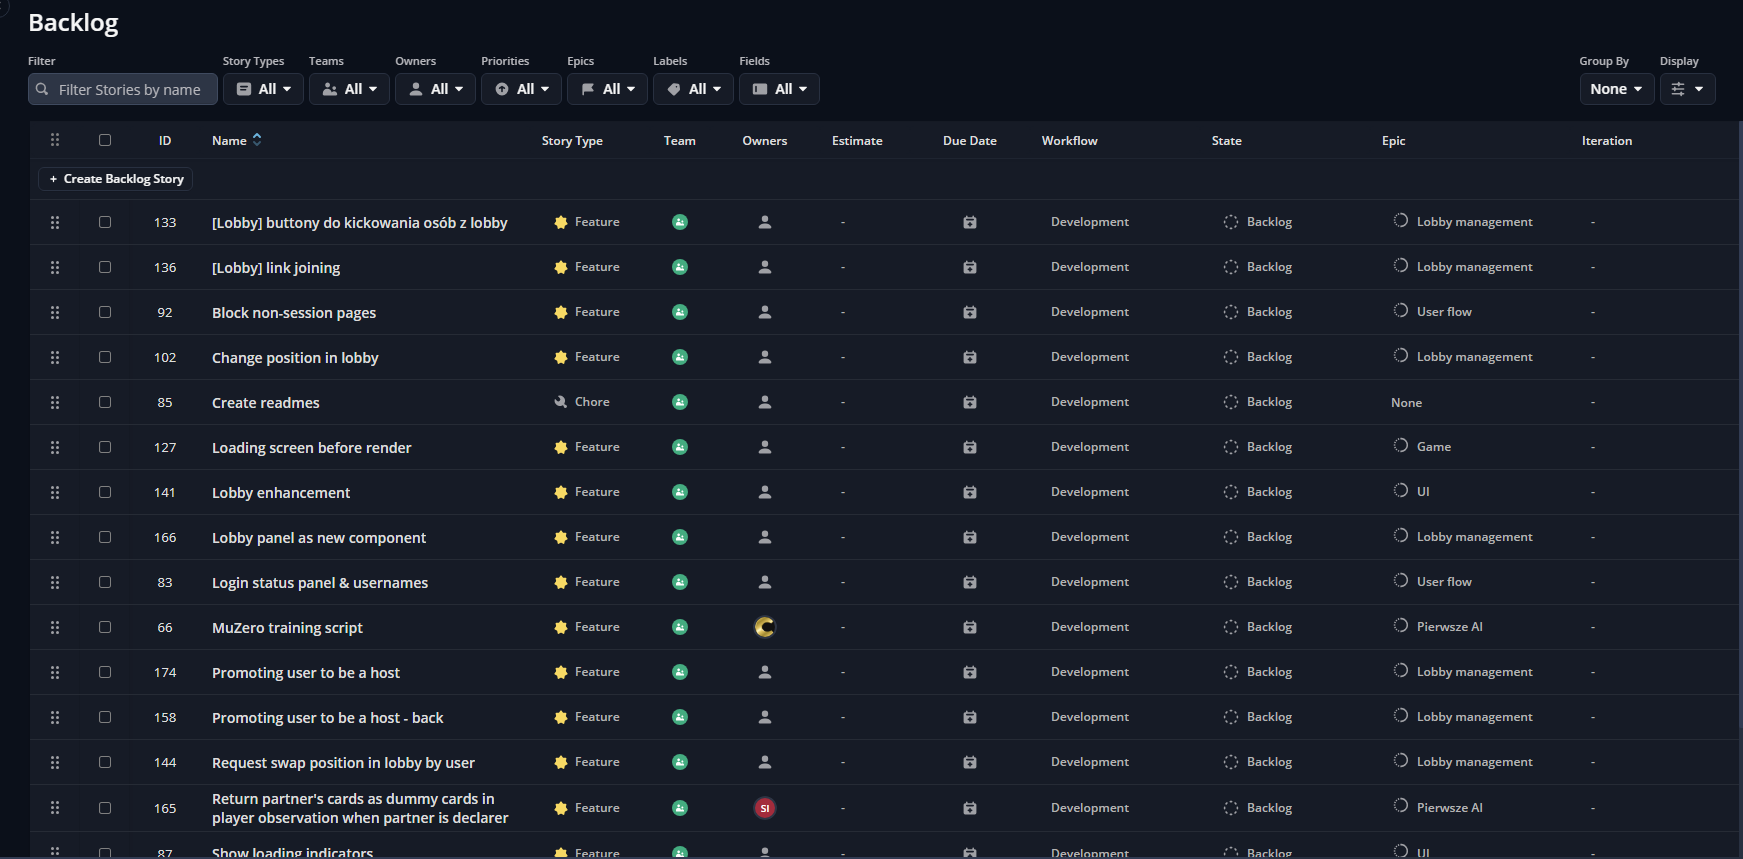
\includegraphics[width=\textwidth]{img/shortcut/shortcut_backlog.png}
    \caption{Backlog z zadaniami}
\end{figure}

\begin{figure}[h]
    \centering
    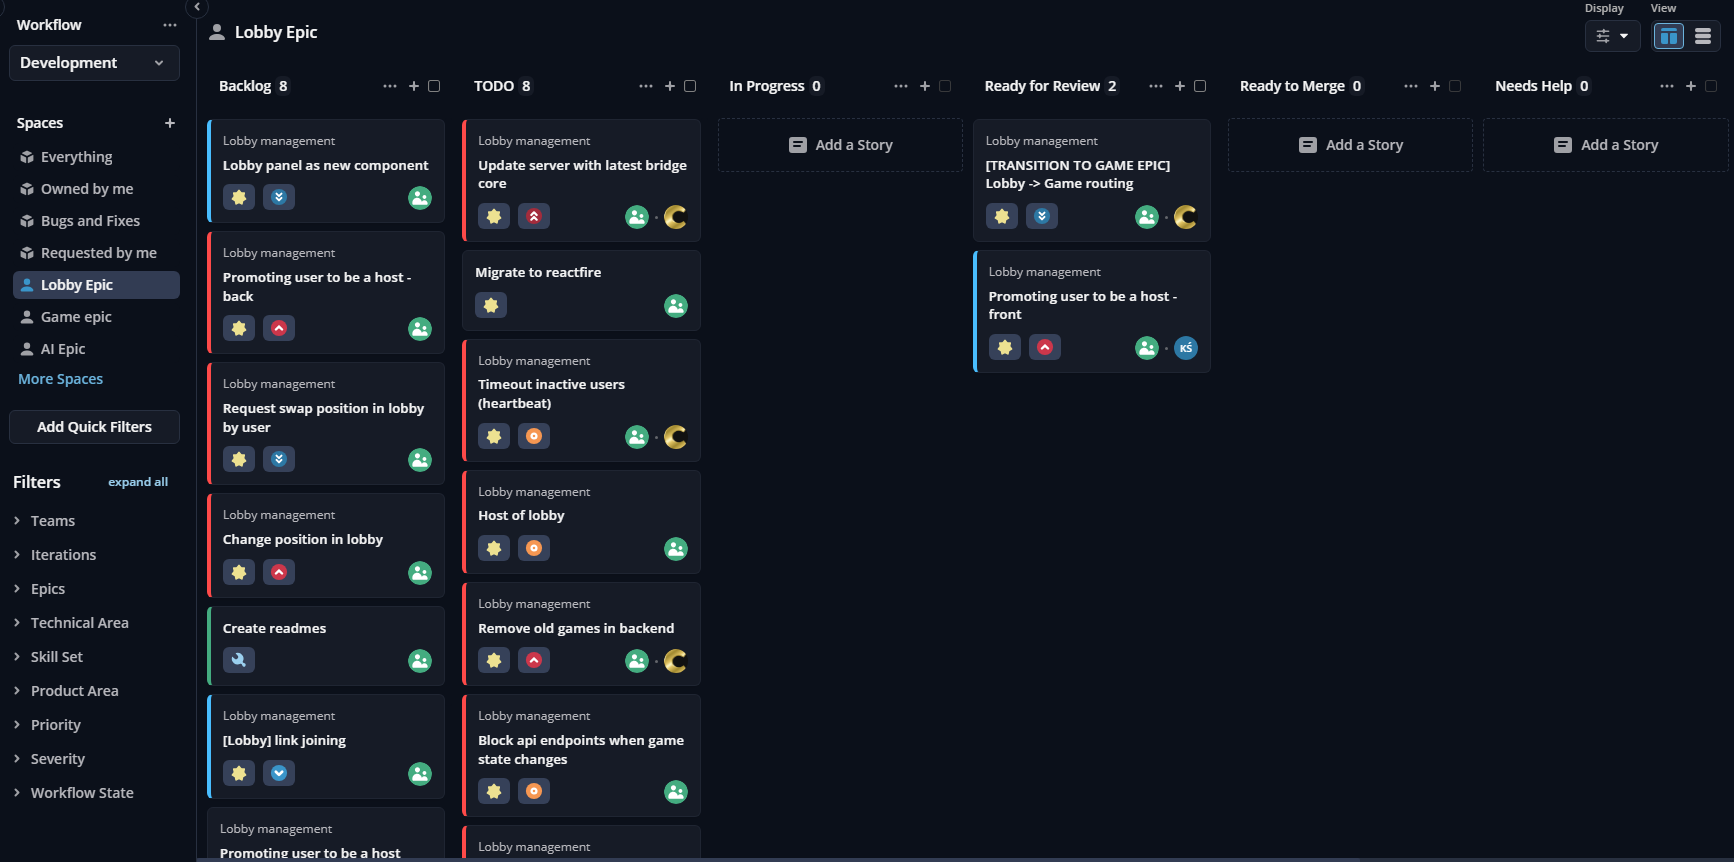
\includegraphics[width=\textwidth]{img/shortcut/shortcut_epic.png}
    \caption{Epic dotyczący systemu lobby wraz z~zadaniami i~ich statusami}
\end{figure}

\FloatBarrier

Również dużym plusem tego rozwiązania była integracja
z~platformą GitHub\cite{Github}, która pozwoliła na
szybkie wyszukiwanie zmian w~kodzie projektu. Poprzez
zastosowane unikalnych identyfikatorów każde zadanie
znajdujące się w~Shortcut mogło mieć odpowiednio przypisaną
zmianę, która zaszła w~projekcie.


\subsubsection{Figma}

Do utworzenia wstępnej wizualizacji aplikacji użyto narzędzie Figma \cite{Figma}.
Służy ono do projektowania graficznego, takich prac jak szkielety stron
internetowych, prototypy interfejsów użytkownika czy też otwartych przestrzeni
do zarządzania i~planowania.

Warto wspomnieć, że tak jak w~\ref{fig:figma_login} lub
\ref{fig:figma_userflow} wykorzystano Figmę do stworzenia mocków i~schematów.

\begin{figure}[h]
    \centering
    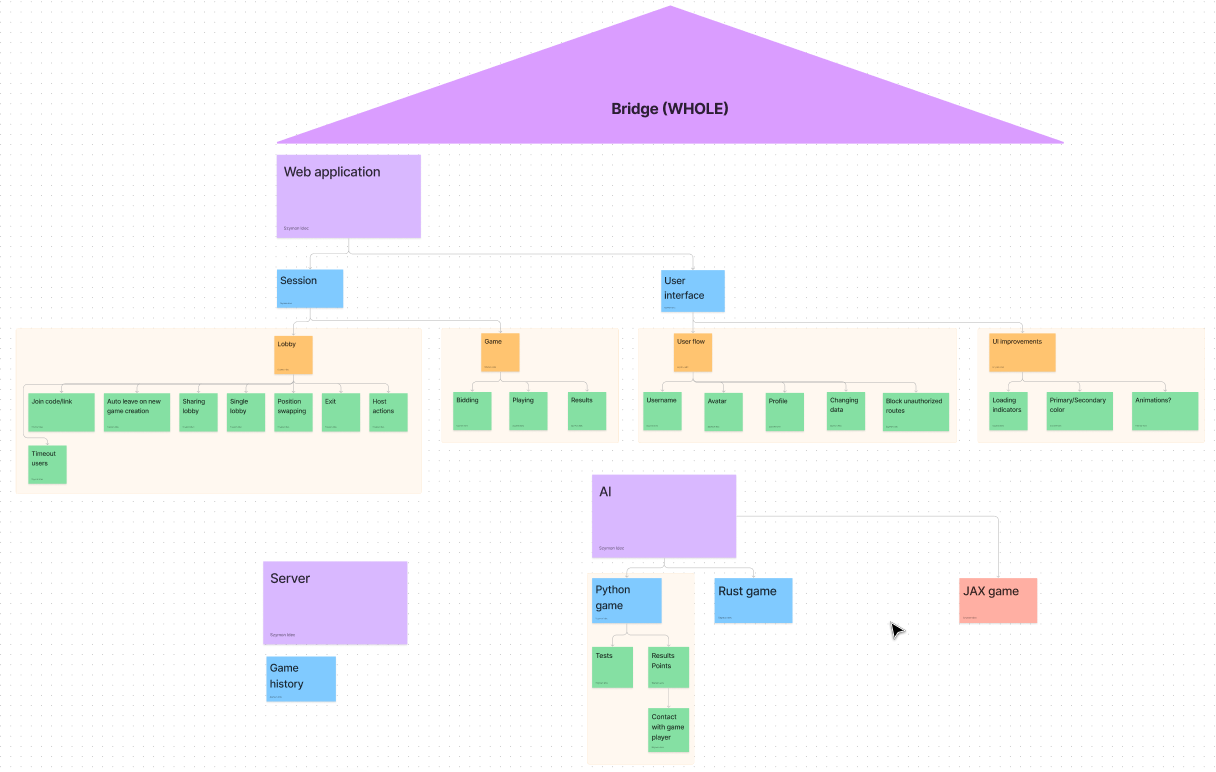
\includegraphics[width=\textwidth]{img/schematy/milestones.png}
    \caption{Szczegółowy podział milestone'ów na zadania}
\end{figure}

\FloatBarrier


\subsection{Komunikacja wewnętrzna}

W~trakcie tworzenia projektu potrzebna była szybka i~efektywna
wymiana wiadomości oraz możliwość współpracy w czasie rzeczywistym.
Wykorzystana została w~tym celu platforma Discord~\cite{Discord},
która oferuje rozmowy głosowe, kanały tekstowe i~udostępnianie
obrazu na żywo.


\subsection{System kontroli wersji}

Aby synchronizować postępy pracy i~ich historię zastosowano
system kontroli wersji Git \cite{Git}. Wraz z~nim, do przechowywania
repozytoriów z kodem aplikacji, jak i~dokumentacji wykorzystano
platformę GitHub.


\subsection{Tworzenie oprogramowania}

Rozwój oprogramowania stanowił kluczowy i~niezbędny element realizacji
założeń projektowych.
Celem było stworzenie funkcjonalnej aplikacji, która integruje
odmienne komponenty, wykorzystujące różne technologie.
W~tym celu skorzystano z~różnych narzędzi, które specjalizowały się
w~tworzeniu i~testowaniu oprogramowania, w~wymaganych przez projekt
technologiach.


\subsubsection{VSCode}

Visual Studio Code \cite{VSCode}, dalej opisywany jako VSCode,
to zaawansowany edytor kodu stworzony
przez Microsoft, który stał się jednym z~najpopularniejszych narzędzi
wśród programistów\cite{IDEIndex}.
VSCode wspiera wiele języków programowania i~znaczników od JavaScript,
TypeScript, Python, C++, Rust po HTML, CSS, JSON i~wiele innych.
Dużą zaletą VSCode jest również możliwość personalizacji. Dostępne są
tysiące rozszerzeń, które pozwalają na dostosowanie edytora do własnych
potrzeb. Użycie tego edytora znacznie usprawniło rozwój aplikacji.

Ze względu na możliwość dostosowania go do różnych języków programowania
i~technologii, stosowano go przy tworzeniu każdego elementu projektu.

Oprócz tworzenia samego oprogramowania w~tym narzędziu wykorzystano go także
do stworzenia dokumentacji aplikacji wraz z~użyciem systemu kontroli wersji Git.
Usprawniło to przebieg pracy nad dokumentem, jak i~wzajemną kontrolę
współtworzenia tekstu.


\subsubsection{Produkty Jetbrains}

Produkty JetBrains \cite{JetBrains}, w~tym dedykowane środowiska
programistyczne (IDE) dla poszczególnych języków i~ekosystemów,
takich jak Java, Python czy PHP.
Oferują one zaawansowane funkcje autouzupełniania i~głębokiej
analizy kodu. Dostarczają one również narzędzia do refaktoryzacji,
co znacząco ułatwia zarządzanie i~optymalizację projektu.

PyCharm \cite{PyCharm}, specjalizujący się w~Pythonie, był pomocny podczas tworzenia
modułu logiki gry w~brydża, a~także w~początkowej fazie konstruowania
serwera z~użyciem FastAPI.

Z~kolei IntelliJ IDEA \cite{Intellij}, ze wsparciem dla języka
Scala, znalazł zastosowanie w~procesie rozwijania ostatecznej wersji
architektury serwerowej.


\subsubsection{Postman}

Postman \cite{Postman} to narzędzie do testowania API, które umożliwia, głównie
programistom i testerom, skuteczne zarządzanie, tworzenie, udostępnianie
i~testowanie żądań HTTP. Jest to popularne środowisko do tworzenia
i~wykonywania zapytań HTTP, zwłaszcza w~kontekście testowania
endpointów RESTful API.

Postman oferuje intuicyjny interfejs graficzny, który ułatwia tworzenie,
wysyłanie i~analizowanie komunikatów sieciowych, a~także sprawdzanie
odpowiedzi serwera. Przydaje się w~wielu etapach procesu tworzenia
aplikacji, od projektowania, wczesnego testowania i~monitorowania API
w~środowisku produkcyjnym.

Przez cały proces tworzenia serwera dla aplikacji Postman był wykorzystywany
do wspomnianych wyżej celów. Było to narzędzie kluczowe w~zapewnieniu
sprawnego działania tej części systemu.


\subsection{Integracja i testowanie}

Podział elementów systemu na wiele części
takich jak aplikacja webowa, serwer, asystent AI
i~dokumentacja wymagał stworzenia odpowiedniego
przepływu pracy zwanego \textbf{CI/CD}. Akronim ten oznacza
ciągłą integrację/ciągłe wdrażanie. Jest on stosowany
w~celu szybkiego likwidowania błędów, przeprowadzania
testów, analizą działania i~integracją elementów systemu
aplikacji. Również pozwala on przyrostowe implementowanie
projektu i~możliwość otrzymania od klienta zwrotnych
informacji o~działaniu systemu.

Zastosowanie tego rozwiązania pozwoliło na
prezentowanie klientowi kolejnych etapów aplikacji, jak
również pozwoliło na niezależne rozwijanie
i~testowanie osobnych części systemu.

Poniżej opisano technologie i~zaprojektowane systemy,
które pozwoliły na skonstruowanie systemu CI/CD dla
tworzonego projektu.


\subsubsection{Github Actions}

Najważniejszym elementem całego systemu było zintegrowanie
repozytorium kodu
wraz z~resztą technologii. Platforma GitHub, na której
znajduje się kod tworzonej aplikacji, oferuje swoje
rozwiązanie GitHub Actions\cite{GithubActions} pozwalające
na zaawansowaną realizację CI/CD. Dla każdego elementu
projektu zostały utworzone instrukcje w~postaci plików JSON
lub wykorzystano integracje zewnętrznych narzędzi oferujące
automatyczne konfiguracje. Instrukcje te były uruchamiane
po aktualizacji kodu.


\subsubsection{Vercel}

\begin{figure}[b!]
    \centering
    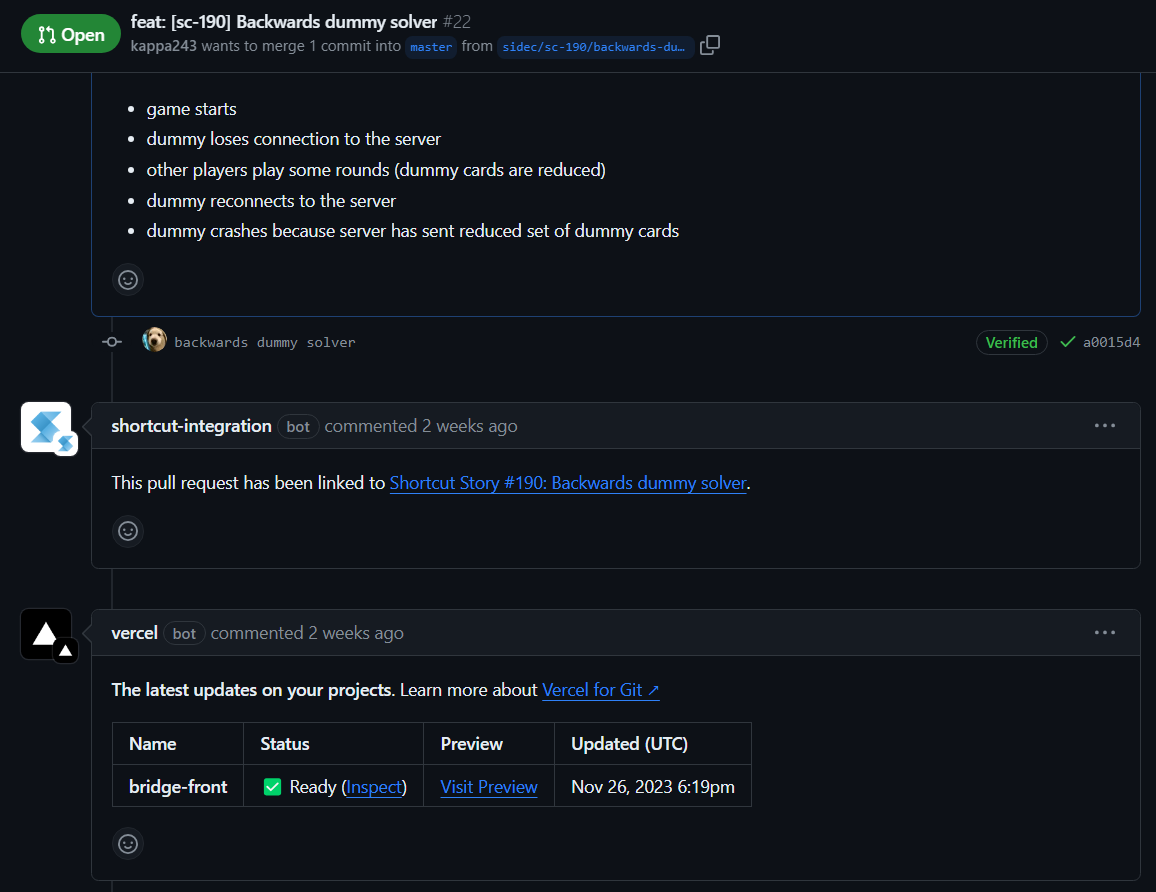
\includegraphics[width=\textwidth]{img/github/github-vercel.png}
    \caption{Wycinek integracji platformy Vercel z~GitHub dla jednej z~gałęzi kodu aplikacji webowej}
    \label{fig:github-vercel}
\end{figure}

Platforma Vercel\cite{Vercel} była odpowiedzialna za
udostępnianie aplikacji webowej. Posiada ona wsparcie \mbox{z~GitHubem},
przez co tworzenie instrukcji odbywa się automatycznie.
Vercel, dla głównej gałęzi kodu \textit{"master"} oraz
gałęzi implementujących dodatkowe funkcje, budował aplikację
i~udostępniał na swojej platformie. W~przypadku aktualizacji
kodu, na odpowiednich gałęziach, przystępował on do ponownego
budowania aplikacji i~zastępował starą. Dla każdej gałęzi
generowany był osobny adres, więc w~przypadku zmian zawsze
najnowsza wersja aplikacji, z~danej gałęzi, była dostępna pod
tym samem odpowiadającym jej adresem. Co więcej, w przypadku
problemów lub błędów podczas budowania aplikacji, informuje
on o~tym i~udostępnienia zapisy logów, aby można było je
zweryfikować. Na rysunku
\ref{fig:github-vercel} można zauważyć, jak dla jednej
z~gałęzi został wygenerowany adres do aplikacji
("Visit Preview") oraz że budowanie przebiegło bez problemów
(zielone zaznaczenie).

\FloatBarrier


\subsubsection{Oracle Cloud}

Do uruchomienia serwera naszego systemu wymagane było
osobne środowisko. Wymagane było, aby oferowało ono
narzędzie do automatycznego budowania i~udostępniania
najnowszych wersji serwera, w~podobny sposób jak zostało
to rozwiązane w~przypadku aplikacji webowej.

Rozwiązano ten problem poprzez stworzenie autorskiego
narzędzia wraz z~wykorzystaniem serwera udostępnionego
przez platformę Oracle Cloud \cite{OracleCloud}.
Wykorzystując możliwość tworzenia instrukcji GitHub Actions
skonfigurowano automatyczne tworzenie obrazu kontenera
Docker \cite{Docker}, który miał za zadanie uruchamiać
serwer. Był on udostępniany w~rejestrze kontenerów na
platformie GitHub. Następnie po stronie serwera Oracle
cyklicznie był sprawdzany rejestr w~celu wykrycia
nowo powstałego obrazu kontenera. Gdy obraz posiadał
inny hash\footnote{hash -- wartość wyliczana przez tzw. "funkcję
    hashującą", która dla otrzymanych na wejściu tych
    samych danych zwraca tę samą wartość.}
odpowiedni skrypt uruchamiał on nową wersję kontenera.
Każda gałąź kodu, podobnie jak w~przypadku aplikacji
webowej, posiadała osobny kontener uruchomiony na serwerze
Oracle. Dzięki temu aplikację webową można było połączyć
z~dowolnie wybraną wersją serwera gry, na przykład, aby
przetestować nową funkcjonalność.


\subsection{Tworzenie dokumentacji}

Do napisania dokumentacji aplikacji użyto języka \LaTeX~\cite{Latex}.
Przesyłając tekst pracy na platformę GitHub, podobnie skorzystano
\mbox{z GitHub Actions}, którą wykorzystano w celu
generacji dokumentu natychmiast po opublikowaniu zmian w~tekście pracy.
Umożliwiło to na dostęp do najnowszej wersji dokumentu dla opiekuna
pracy i~prowadzącego pracownię projektową, dzięki czemu była możliwa
ciągła weryfikacja postępów nad pracą.

